\documentclass[]{itmo-student-thesis}

\usepackage[utf8]{inputenc}
\usepackage{amsmath,amssymb}
\usepackage[russian]{babel}
\usepackage{multirow}

\usepackage{graphicx}
\graphicspath{ {images/} }
\selectlanguage{russian}

\newcommand{\todo}[1]{\vspace{5 mm}\par \noindent
\marginpar{ToDo}
\framebox{\begin{minipage}[c]{0.95 \textwidth}
    \tt #1 \end{minipage}}\vspace{5 mm}\par}

\addbibresource{bachelor-thesis.bib}

\begin{document}

\studygroup{M3439}
\title{Построение векторного представления предложения с использованием дерева синтаксического разбора}
\author{Пересадин Илья Валерьевич}{Пересадин И.В.}
\supervisor{Путин Евгений Олегович}{Фильченков А.А.}{к.ф-м.н., доцент кафедры КТ}{}
\publishyear{2017}


%% Эта команда генерирует титульный лист и аннотацию.
\maketitle{Бакалавр}

% Оглавление
\tableofcontents

% Chapters
\startprefacepage
В нашу эпоху современных технологий, человек пытается максимально
роботизировать все процессы нашей жизни. Ученые работают над тем,
чтобы компьютер без проблем понимал, что от него хочет пользователь и с легкостью
решал поставленные задачи. 
Для того, чтобы компьютер мог понимать человеческий язык, было изобртено направление искусственного интеллекта~--- обработка естественного языка (от англ. Natural Language Processing). 
NLP изучает проблемы анализа и синтеза естественных языков\cite{wikinlp}.
Большую нишу NLP заняли искусственные нейронные сети.

Искусственные нейронные сети (ИНС) являются одним из мощных инструментов машинного
обучения.
Это математическая модель, которая работает подобно тому, как работает головной
мозг человека \cite{rosenblatt58a}.
Они были изобретены в 60-х годах предыдущего века, и нашли свое активное
применение в наши дни. Конечно ИНС претерпевали изменения и модернизации, было разработано множество архитектур, а также алгоритмов обучения\cite{Duchi2011, zeiler2012, rprop93}.

%Актуальность
Важной задачей NLP является задача  обработки и 
извлечения семантического содержимого предложения (sentence modelling).
Она используется для создания чат-ботов, переводов текстов (machine translation), 
извлечение фактов из текста (information extraction), схожесть утверждений (semantic relatedness), 
а также различных классификаций текстов, например, по стилю или по эмоциональному тону (sentiment analysis).
В частности, широкое распространение получили методы, 
которые сопоставляют предложению некоторый вещественный вектор, 
с помощью которого и происходит анализ предложения.

%Новизна
В данной работе будет предложена модель, вычисляющая векторное представление предложения, 
которая использует \emph{дерево синтаксического разбора} (syntactic parse tree) предложения, а также учитывают локальный контекст каждого слова предложения.
На данный момент не существует решений, которые явно учитывают оба этих аспекта.
Также будет предложен новый подход вычисления векторного представления предложения.

% Структура работы
В главе 1 будут введены вспомогательные понятия, сформулированы решаемые задачи.
Будут рассмотрены существующие решения на основе \emph{cверточных нейронных сетей} (от англ. Сonvolutional Neural Networks или CNN), \emph{рекурсивных нейронных сетей} (от англ. Recursive Neural Network или RNN), а также такие решения как Paragraph Vector и \emph{рекурсивная тензорная нейронная сеть} (от англ. Recursive Neural Tensor Network или RNTN).

В главе 2 будут рассмотрены предложенные улучшения, их принцип работы и обоснование.

В главе 3 будут рассмотрены результаты, достигнутые предложенными решениями на задачах классификации
эмоционального тона предложения и задача классификации вопросов, а также сравнение с существующими решениями.

%-*-coding: utf-8-*-

\chapter{Обзор предметной области}

\section{Постановка задачи}
\noindent Пусть есть некоторый язык со словарем $V$.\\
Пусть есть некоторая функция ошибки $L:\mathbb{R}^s \to \mathbb{R}$.\\
Пусть $D$~--- множество последовательностей над $V$, называемое датасетом задачи.\\
Задача построения векторного представления предложения, состоит в изобретении такой модели $M$, 
которая для любой последовательности слов $w \in V^n$ (любому предложению) сопоставляет
вектор $M(w) \in \mathbb{R}^s$ так, что суммарная ошибка $$\sum_{w \in D} L(M(w))$$ была как можно меньше.
Чем меньше эта ошибка, тем более качественна модель $M$.\\

\section{Решаемые задачи}
В данной работе будет предложена модель, качество которой будет оценено на задачах классификации эмоционального тона предложения и классификации вопросов.
\vspace{5mm}

\noindent \textbf{Задача классификации эмоционального тона предложения}\par
Задача классификации эмоционального тона предложения состоит в оценке эмоциональной характеристики предложения. Например, в данной работе будут рассмотрены датасеты, которые содержат обзоры фильмов. Предложенная модель должна будет предсказать, какому из пяти эмоциоанльных классов относится обзор:
\emph{очень негативный}, \emph{негативный}, \emph{нейтральный}, \emph{позитивный}, \emph{очень позитивный}.
\vspace{5mm}

\noindent \textbf{Задача классификации вопросов}\par
Задача классификации вопросов состоит в определении к какому типу принадлежит вопрос:
аббревиатура, сущность (животное, еда и т.д), описательный, личность, расположение, числовой.

Данные классы включают в себя более точные подклассы, на которых также будет проведена оценка модели.

\section{Вспомогательные понятия}

\subsection{Векторное представление слов}
Векторное представление слова (word embedding)\cite{Bengio03aneural}~--- параметризованное отображение слова на пространство большой размерности $\mathbb{R}^d$. 
Такое представление сохраняет семантические отношения между словами. 
Причем, похожим словам сопоставляются близкие по некоторой метрике вектора, 
а различным~--- удаленные друг от друга.

Векторное представление слов либо обучают <<с нуля>> вместе с основной моделью, либо берут за основу предобученные на достаточно большом корпусе текстовых данных. Наиболее крупные корпусы векторных представлений это word2vec\cite{DBLP:journals/corr/MikolovLS13, wor2vec}, а также GloVe\cite{pennington2014glove, glove}, которые также будут использоваться в данной работе.

\subsection{Дерево синтаксического разбора предложения}
Существует несколько способов построения дерева синтасксического разбора.
Это зависит от принципов построения и сущностей, которые поддерживает дерево зависимостей.
Так, например, существуют Stanford Dependencies\cite{standeps}, а также Universal Dependencies\cite{unideps}.
В данной работе будет использоваться преимущественно способ Probabilistic Context-Free Grammars\cite{pcfg}.

Данный способ задается грамматикой, по которой и разбирается предложение\cite{Klein03accurateunlexicalized}.
По языку строятся подкатегории фраз, например, такие как "noun phrase" (NP), "verb phrase" (VP) и т.д. 
Для них также строятся правила вывода грамматики. После чего предложение разбирается по этим правилам. 

\begin{figure}[h]
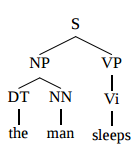
\includegraphics[scale=1.0]{pcfgs}
\caption{\textbf{Пример разбора предложения PCFG парсером}}
\label{fig:pcfgs}
\end{figure}

Данная граматика может быть неоднозначна, 
поэтому вывод происходит вероятностно~--- выбирается наиболее вероятное правило в данном контексте.

Вообще говоря, предложенная модель не зависит от способа построения дерева разбора и языка.

\section{Обзор существующих решений}

В данной главе будут приведены существующие решения для построения векторного представления предложения.

\subsection{Paragraph Vector}
Целью подхода Paragraph Vector является сопоставление вещественного вектора в $\mathbb{R}^d$ последовательности слов произвольной длины: предложению, абзацу или даже документу\cite{DBLP:journals/corr/LeM14}.
Paragraph Vector учитывает семантический контекст текста на котором он получен.

Параметрами Paragraph Vector являются: вещественная матрица $W$~--- векторное представление слов словаря текстового корпуса, а также вещественная матрица $D$~--- векторное представление абзацев корпуса. Метод пытается предсказать следующее слово в абзаце, опираясь на векторное представление данного абзаца, а также слов из абзаца, смежных с предсказываемым словом, то есть находящихся в одном контексте с ним.
Данный метод может быть также применен к предложению.

\begin{figure}[h]
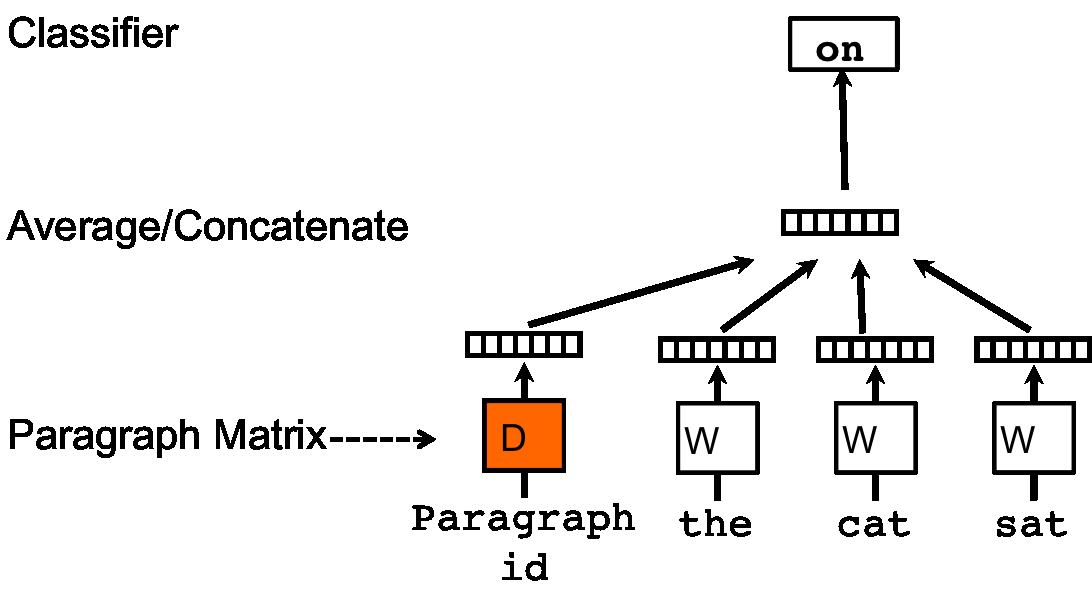
\includegraphics[scale=0.65]{par_vec}
\caption{\textbf{Paragraph Vector}}
\label{fig:par_vec}
\end{figure}

\subsection{Рекуррентная нейронная сеть}
Основным инструментом для обработки текстов являются так называемые \emph{рекуррентные нейронные сети}(РНС)\cite{Goller96learningtask-dependent}.

Рекуррентные нейронные сети предназначены (РНС) для обработки последовательных данных, таких как звук и текст. В традиционных нейронных сетях все входы считаются независимыми друг от друга, но для многих задач это не так, и такой подход не учитывает много информации о структуре данных.

РНС принимает слова последовательности поочереди, сохраняя внутри себя контекст уже принятого текста. Рекуррентными они называются потому что выполняют одну и ту же задачу для каждого слова в тексте. Данная архитекутра достаточно хорошо отражает процесс восприятия информации человеком: после того как мы прочли начало предложение, в нашей голове уже сформировался некоторый контекст, и следующее слово обрабатывается нами с учетом уже прочитанной информации, а не воспринимается с чистого листа.

\begin{figure}[h]
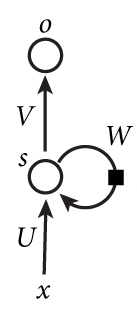
\includegraphics[scale=0.7]{rnn}
\caption{\textbf{РНС}}
\label{fig:rnn}
\end{figure}

\begin{figure}[h]
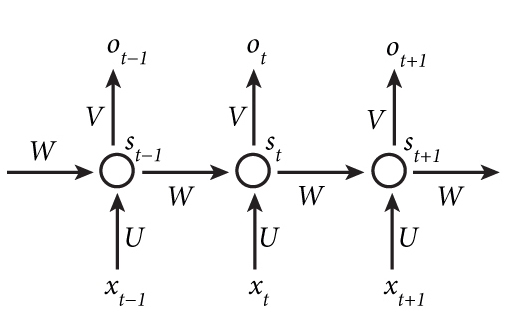
\includegraphics[scale=0.7]{rnn-unfold}
\caption{\textbf{РНС в развернутом виде}}
\label{fig:rnn-unfold}
\end{figure}

\noindent $U, W, V$~--- параметры РНС сети\\
$x_t$~--- вектор, соответствующий слову $t$ \\
$s_t$~--- информация о первых $t$ словах \\
$o_t$~--- выходной вектор

Хотя РНС является достаточно мощной моделью, у нее есть ряд недостатков, самый большой из которых~--- это так называемая <<проблема затухания градиента>>. Суть ее заключается в том, что РНС не может запоминать контекст начала предложения в длинных последовательностях слов. Поэтому на смену РНС была изобретена другая архитектура РНС, под названием \emph{долгая краткосрочная память} (ДКП) (от англ. Long Short Term Memory или LSTM), которая решает эту проблем\cite{Hochreiter:1997:LSM:265493.264179}. Одна ячейка ДКП:
$$i_t=\sigma \left( W^{(i)}x_t+U^{(i)}h_{t-1} + b^{(i)} \right)$$
$$f_t=\sigma \left( W^{(f)}x_t+U^{(f)}h_{t-1} + b^{(f)} \right)$$
$$o_t=\sigma \left( W^{(o)}x_t+U^{(o)}h_{t-1} + b^{(o)} \right)$$
$$u_t=\tanh \left( W^{(u)}x_t+U^{(u)}h_{t-1} + b^{(u)} \right)$$
$$c_t=i_t \odot u_t + f_t \odot c_{t-1}$$
$$h_t=o_t \odot tanh(c_t)$$
где $W^{(i)}, W^{(f)}, W^{(o)}, W^{(u)} \in \mathbb{R}^{a \times h},\\U^{(i)}, U^{(f)}, U^{(o)}, U^{(u)} \in \mathbb{R}^{h \times h},\\b^{(i)}, b^{(f)}, b^{(o)}, b^{(u)} \in \mathbb{R}^{h}$~--- параметры модели\\
$x_t \mathbb{R}^a$~--- one-hot вектор $t$-го слова предложения

Таким образом, на вход ДКП подается предложение и в качестве векторного представления используется
последний вектор $h_n$.

\subsection{Сверточная нейронная сеть}
Сверточная нейронная сеть (СНС)~--- успешно показала себя в обработке и анализе изображений. Они работают подобно тому, как происходит распознавание образов в головной коре человека. СНС состоят из нескольких слоев, каждый из которых детектирует некоторые визуальные признаки изображения, такие как прямые линии, окружности. Признаки с предыдущего слоя используются для формирования более высокоуровневых визуальных признаков.

Преимуществом СНС является выделение локалных пространственных признаков. В контексте изображений это означает, что визуальные признаки локализуются сначала на неболших квадратах, а далее объединяются в большие фигуры.

Оказывается, данный плюс можно использовать и для построения векторного представления, 
если рассмотреть слова предложения как вектора некоторой размерности. Тогда если в предложении $n$ слов, 
и размерность векторного представления слова $d$, получаем матрицу $n \times d$, 
которую можно трактовать как изображение и применить к нему сверточную нейронную сеть\cite{Lecun98gradient-basedlearning, DBLP:journals/corr/Kim14f}.

\begin{figure}[h]
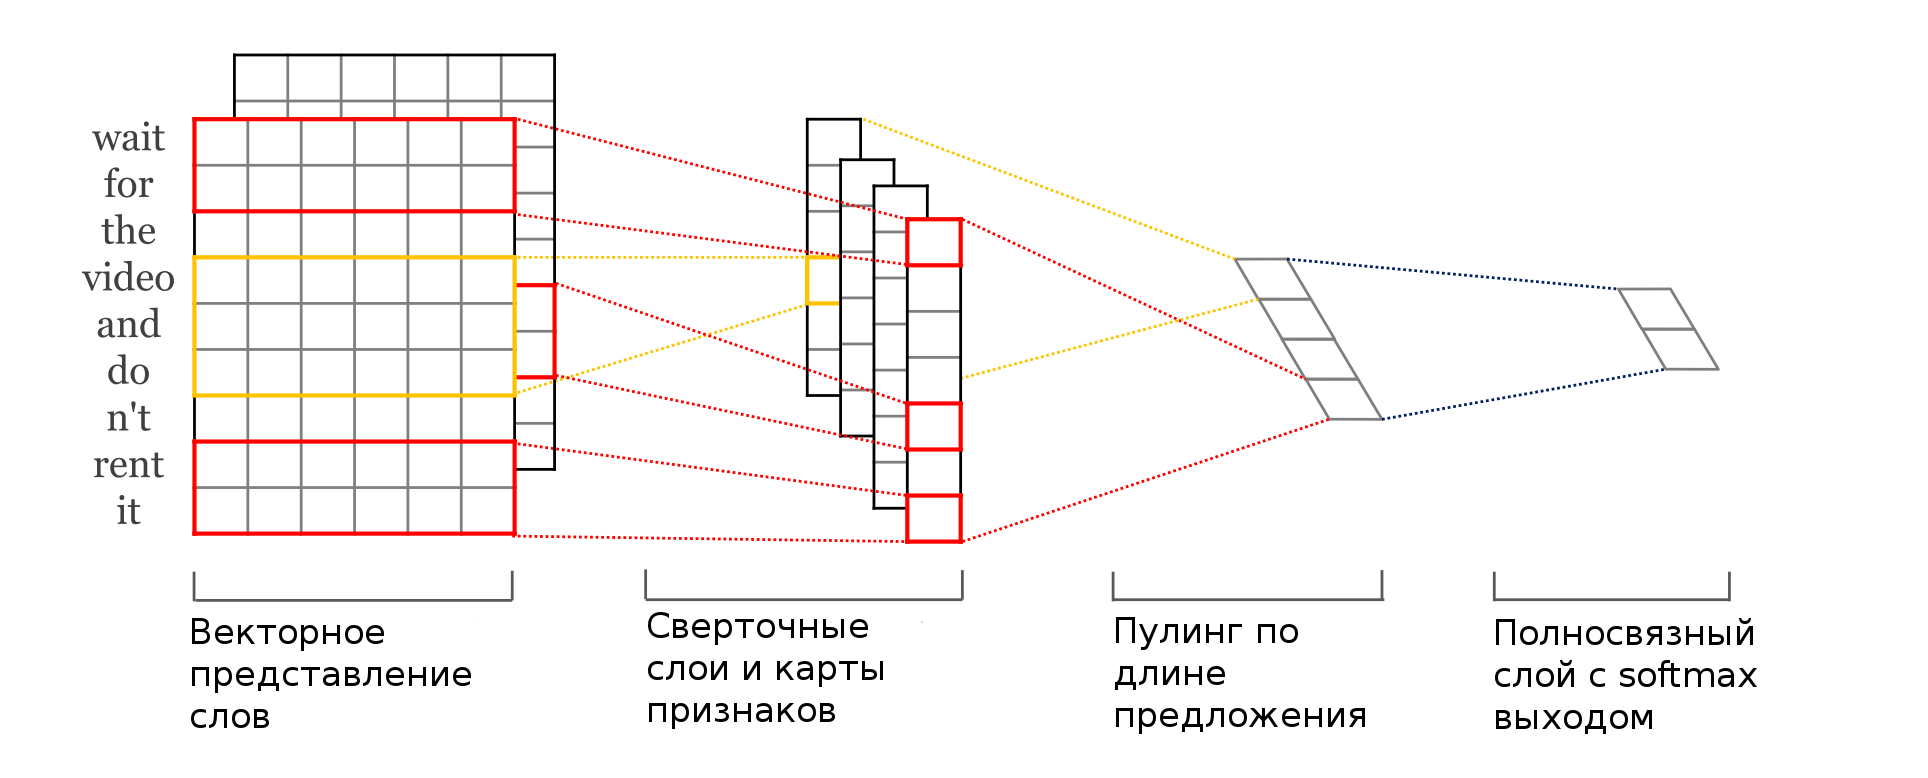
\includegraphics[scale=0.55]{cnn-rus}
\caption{\textbf{СНС для предложения}}
\label{fig:cnn}
\end{figure}

\subsection{Рекуррентная тензорная нейронная сеть}
Еще одним важным подходом для построения векторного представления является использование 
дерева синтаксического разбора предложения. Вообще говоря, решения, использующие этот подход, предполагают, что у предложения уже построено дерево синтаксического разбора. Построение дерева является отдельной достаточно важной задачей NLP. На данный момент существуют алгоритмы, которые делают это построение с очень хорошей точностью[статьи]. 
С другой стороны, обычно для таких решений не столь важно точное построение дерева, то есть они не критичны к неточностям в дереве разбора.

Рекуррентная тензорная нейронная сеть (РТНС)~--- одно из решений, использующее дерево синтаксического разбора. Целью данного метода является сопоставление каждой вершине дерева разбора вектора в $\mathbb{R}^d$, 
который и характеризует семантическое содержание фразы, соответствующей поддереву этой вершины.
Вектор для вершины $p$ вычисляется как $f(p)=g(f(c_1), f(c_2) \dots{} f(c_k))$, где $c_i$~--- непосредственные потомки вершины $p$, а $g$~--- некоторая функция. Вычисление происходит снизу-вверх, то
есть от листьев дерева к его корню. Для листьев $f(p)$ берутся произвольными и улучшаются в результате обучения в соответствии с поставленной задачей.
В качестве функции $g$ в оригинальной работе\cite{socher-EtAl:2013:EMNLP} используется умножение на $n$-мерный тензор.

\begin{figure}[h]
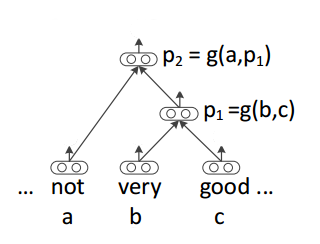
\includegraphics[scale=0.7]{rntn}
\caption{\textbf{Рекуррентная тензорная нейронная сеть}}
\label{fig:rntn}
\end{figure}
%-*-coding: utf-8-*-

\chapter{Описание предложенного решения}

В данной главе будут рассмотрены предложенные идеи архитектур нейронных сетей на основе дерева разбора предложения.

В разделе 2.1 будут кратко описаны предложенные идеи и мотивация их использования.

В разделе 2.2 будет дано формальное описание модели.

\section{Предложенные идеи}

\subsection{Контекст слов в предложении}

Минусом подхода РТНС является то обстоятельство, что для поддеревьев с небольшим количеством слов (до 4-5 слов), методу сложно построить векторное представление достаточно точно, ввиду отсутствия контекста использования слов. 
Так, в данном примере:

\todo{Пример}

Данная проблема наталкивает на мысль учитывать слова, 
использующиеся вместе с каждым словом в предложении, перед передачей в РНТС.

\subsection{Значимые слова в предложении}
Еще одной проблемой существующих решений, является то,  что они учитывают все слова предложения, 
хотя достаточно большое количество слов не несет смысловой нагрузки для решаемой задачи, а также для построения взаимосвязей
между словами.
Это требует от модели более избирательного анализа слов, а также порождает проблему \textquote{затухания градиента}, из-за 
длинной последовательности вычислений.

Рассмотрим следующий примеры для задачи классификации эмоционального тона предложения на датасете, состоящем из
обзоров кинофильмов.

{\fontfamily{cmss}\selectfont A \textbf{screenplay more ingeniosly} constructed \textbf{than Memento}.}

{\fontfamily{cmss}\selectfont Suffers from the \textbf{lack} of a \textbf{compelling} or \textbf{comprehensible narrative}.}

{\fontfamily{cmss}\selectfont Still, this \textbf{flick is fun} and \textbf{host to} some truly \textbf{excellent sequences}.}

\noindent Жирным выделены слова, которе несут основную смысловую нагрузку предложения.\\
Можно видеть, что достаточно большой процент от общего количества слов в предложении составляют 
\textquote{незначимые} для задачи слова.

Данная идея как раз и состоит в выделении наиболее значимых слов и фраз в предложении.
Эту идею можно обобщить на дерево разбора.

\section{Формальное описание алгоритма}

\subsection{Предобработка данных}
Для того чтобы алгоритм смог проанализировать предложение, 
его необходимо привести к определенному формату. Мы рассмотрим обработку
тренировочных данных, обработка тестовых данных производится аналогично.

В первую очередь, предложение необходимо разбить на слова. 
Это можно сделать используя регулярные выражения. 

Затем по данному корпусу предложений необходимо построить словарь слов.
Словарь~--- это некоторое подмножество слов предложений корпуса.
Это делается для того, чтобы ограничить объем вычислений, так как использование всех
слов языка достаточно ресурсоемко. Обычно в словарь попадают слова, 
имеющие наибольшую частоту использования в данном корпусе, 
либо просто все слова корпуса.

Те слова из корпуса, которые не попали в словарь заменяются специальным словом $UNK$, 
оно также добавляется в словарь.

Затем каждому слову $w$ из словаря сопоставляется целочисленный индекс $i_w$ 
от $0$ до $N-1$, где $N$~--- размер словаря.
Каждое слово в словаре задается вектором размерности $N$, 
в котором на позиции $i_w$ находится единица, а на остальных позиция~--- нули
Оперированием данным вектором напрямую также ресурсоемко, поэтому вводится вещественная матрица $W$, 
размерности $N \times d$, где $N >> d$. Тогда вектор для слова $w$ вычисляется как
$$a_w = E_{i_w} \cdot W$$
где $E$~--- единичная матрица $N \times N$.
Таким образом мы построили векторное представление для слов из словаря, которое задается матрицей $W$.

Матрица $W$ является обучаемым параметром, и инициализируется либо произвольными числами, 
либо же используются предобученные на больших корпусах данных векторные представления, 
такие как $word2vec$ или $GLoVe$ [ссылки].

Теперь необходимо для предложения построить дерево синтаксического разбора.
В рамках данной работы мы будем делать это, используя готовое решение $Stanford$ [ссылка].

При тестировании модели, производится аналогичная предобработка, 
с тем лишь отличием, что используется словарь, построенный по тренировочным данным.

Заметим, что весь процесс предобработки предложений автоматизирован, 
и не требует вмешательства человека.

\subsection{Описание идеи \textquote{локальный контекст слов}}

Формально, предложение задается матрицей в  $\mathbb{R}^{l \times{} d}$, в которой $i$-я строка равна векторному представлению слова на позиции $i$,\\
где $l$~--- количество слов в предложении,\\
$d$~--- размерность векторного представления слов. 

Наша задача: получить новую матрицу в $\mathbb{R}^{l \times {} t}$, где $i$-я строка задает векторное представление \textit{контекста} данного слова в предложении. 
Данная операция задается оператором $F:\mathbb{R}^{l \times d} \to \mathbb{R}^{l \times t}$.

В рамках данной работы мы рассмотрим такие операторы $F$, которые в качестве контекста
для слова $i$ используют смежные слова.\\
Формально: слова, на таких позициях $j$, что $i \le j < i + k$, где $k \in \mathbb{N}$~--- фиксированное значение и является параметром алгоритма.\\Оператор такого вида определяется оператором
$C:\mathbb{R}^{k \times d} \to \mathbb{R}^t$, который определяет способ 
получить векторное представление из смежных слов. \\
Тогда $$F(X)_i = C(X'_{i..i+k-1})$$
где $X'$~--- это $X$ c добавленными в конец $k-1$ строками из нулей, \\
$X'_{i..i+k-1}$~--- матрица, образованная строками $X'$ c $i$ по $i+k-1$.\par

\vspace{5mm}

\noindent В данной работе будут использоваться следующие операторы $C$:
\begin{itemize}
    \item{полносвязный слой}
        $$C_{FC}(X)=\sigma(X^T \cdot W + b)$$
        где $W \in R^k, b \in R^d$, в данном случае $t=d$
    \item{сверточная нейронная сеть}
        $$c_j(X)=\sigma(X \odot m_j + b_j)$$
        $$C_{CNN}(X)=[c_1(X); c_2(X); \cdots c_t(X)]$$
        где $m_j \in \mathbb{R}^{k \times d}, b_j \in \mathbb{R}$,\\
        $\odot$~--- поэлементное произведение и суммирование полученных произведений, 
        так называемая операция \textquote{свертки}
    \item{долгая краткосрочная память}
    $$h_i=LSTM_h(c_{i-1},h_{i-1}, X_i) \text{ для } i \text{ от } 1 \text { до } k$$  
    $$c_i=LSTM_c(c_{i-1}, h_{i-1}, X_i) \text{ для } i \text{ от } 1 \text { до } k$$ 
    $$c_0 = \emptyset, h_0 = \emptyset$$
    $$C_{LSTM}(X) = h_k$$
    где $LSTM$~--- ячейка долгой краткосрочной памяти, описанной в разделе[]\\
    $LSTM_h, LSTM_c$~--- вычисление векторов $c$ и $h$ из $LSTM$ ячейки соответственно,\\
    $h_i \in \mathbb{R}^t, c_i \in \mathbb{R}^t$
\end{itemize}

\noindent Эта идея была названа \textquote{локальный контекст слов}.

\subsection{Описание идеи \textquote{значимые поддеревья}} 

Перед нами стоит задача: вычислить для каждой вершины дерева разбора 
векторное представление фразы, соотвествующей этой вершине.
Мы будем делать это восходящим образом, вычисляя векторное представление для листьев,
затем для их предков, и так далее до корня дерева.

Обозначим векторное представление вершины $v$ за $f_v \in \mathbb{R}^s$.
Для вычисления $f_v$ в поддереве вершины $v$ будем выбирать такие поддеревья, 
что соответствующие им фразы являются наиболее значимыми для решаемой задачи.

Введем для каждой вершины $u$ весовой вектор $w_u \in \mathbb{R}^p$  так, что
чем больше квадрат нормы  этого вектора, тем более значима фраза, соотвествующая $u$.

Теперь чтобы посчитать векторное представление вершины $v$, выберем $K(v)$ вершин
в ее поддереве с наибольшими значениями $\lVert w_u \rVert^2$, пусть это $\{ u'_1, u'_2, \dots u'_{K(v)} \}$.
Затем с помощью некоторого оператора $G_v:\mathbb{R}^{K(v) \times s} \to \mathbb{R}^s$, 
передав в него выбранные значения $f_{u'_i}$, посчитаем векторное представление $f_v$.
Теперь остается пересчитать $w_v$. Сделаем это аналогичным образом, используя некоторый оператор 
$W_v :\mathbb{R}^{K(v) \times (s + p)} \to \mathbb{R}^p$, $f_{u'_i}$ и $w_{u'_i}$.

Формально:
$$TopK_v \{ \lVert w_{u_1} \rVert^2, \lVert w_{u_2} \rVert^2, \dots, \lVert w_{u_{2n-1}} \rVert^2\} = \{u'_1, u'_2, \dots, u'_{K(v)}\}$$
$$f_v = G_v(f_{u'_1}, f_{u'_2}, \dots, f_{u'_{K(v)}})$$
$$w_v = W_v(f_{u'_1} \circ w_{u'_1},f_{u'_2} \circ w_{u'_2}, \dots, f_{u'_{K(v)}} \circ w_{u'_{K(v)}})$$

\noindent $n$~--- количество слов в фразе, соответствующей вершине $v$\\
$u_1, u_2, \dots u_{2n-1}$~--- вершины поддерева $v$ в порядке эйлерова обхода\\
$TopK_v$~--- функция, которая выбирает $K(v)$ наибольших значений и возвращает их порядковые номера\\
$K(v)$~--- функция, которая определяет количество значимых поддеревьев для вершины $v$\\
$\circ$~--- операция конкатенации двух векторов в один

Мы можем видеть, что данный подход задается семействами операторов $G_v$ и $W_v$, и функцией $K$.

\todo{Что используется в качестве K}

\noindent Эта идея была названа \textquote{значимые поддеревья}.

\subsection{Архитектура и обучение модели}

Архитектуру полученной модели можно условно разбить на три части
\begin{enumerate}
    \item{подсчет векторного представления локального контекста}
    \item{подсчет векторного представления поддеревьев}
    \item{способ решение поставленной задачи по векторному представлению корня}
\end{enumerate}

Первый пункт был формально описан в разделе 2.2.2[].

Раздел 2.2.3 описывает предложенный механизм для подсчета векторного представления поддеревьев.
Помимо предложенного решения, в рамках данной работы используется простая рекуррентная модель пересчета поддеревьев [статья], которая задается как:
$$f_v = \sigma(f_l \cdot W_1 + f_r \cdot W_2 + b)$$
где $f_v$~--- векторное представление вершины $v$, а $f_l$ и $f_r$~--- непосредственных
потомков веришы $v$,\\
$W_1, W_2 \in \mathbb{R}^{s \times s}$,
$b \in \mathbb{R}^s$~--- параметры рекуррентной модели

А также, древовидная LSTM модель [статья], которая задается как:
$$\tilde{i}_v=\sigma \left( U_1^{(i)} \cdot h_{v,1} + U_2^{(i)} \cdot h_{v,2} + b^{(i)} \right)$$
$$\tilde{f}_{vk}=\sigma \left( U_1^{(f)} \cdot h_{v,1} + U_2^{(f)} \cdot h_{v,2} + b^{(f)} \right),\text{ }k=1,2$$
$$\tilde{o}_{v}=\sigma \left( U_1^{(o)} \cdot h_{v,1} + U_2^{(o)} \cdot h_{v,2} + b^{(o)} \right)$$
$$\tilde{u}_{v}=\tanh \left( U_1^{(u)} \cdot h_{v,1} + U_2^{(u)} \cdot h_{v,2} + b^{(u)} \right)$$
$$\tilde{c}_v=\tilde{i}_v \odot \tilde{u}_v + \tilde{f}_{v,1} \cdot \tilde{c}_{v, 1} + \tilde{f}_{v,2} \cdot \tilde{c}_{v, 2}$$
$$\tilde{h}_v=\tilde{o}_v \cdot \tanh(\tilde{c}_v)$$

Способ решения задачи по векторному представлению корня непосредственно зависит от самой задачи.
В рамках данной работы нам потребуется решать задачу классификации предложений по эмоциональному тону.
Для нее будет использоваться полносвязный слой c последующей softmax-функцией активации. 
В качестве функции потери используется кросс-энтропийная функции ошибки. Формально:
$$z=f_{root} \cdot W_{out} + b_{out}$$
$$\tilde{y}_j=\frac{e^{z_j}} {\sum_{k=1}^K e^{z_k}}$$
$$L_2 = \sum_i y_i \cdot \log(\tilde{y_i})$$
где $f_{root} \in R^s$~--- векторное представление корня,\\
$K$~--- количество классов в задаче классификации\\
$W_{out} \in \mathbb{R}^{s \times K}, b_{out} \in \mathbb{R}^K$~--- параметры полносвязного слоя\\
$y_j$~--- правильный ответ для данного входного примера\\
$\tilde{y}_j$~--- распределение вероятностей по классам задачи классификации, сгенерированное моделью\\
$L_2$~--- значение ошибки на данном входном примере

Отметим, что обучение каждой части модели происходит вместе, а не пораздельности. 
Так, например, если требуется использовать данный подход для переводов текстов, 
то векторное представление корня передается в декодер[статья], 
параметры которого обучаются вместе с параметрами модели.
\subsection{Архитектурные решения}
 
%-*-coding: utf-8-*-

\chapter{Эксперименты и результаты}
 
\subsection{Описание наборов данных и методики тестирования}
 
Предложенное решение было протестировано на нескольких задачах. 
Наборы данных содержат синтаксические деревья либо предложения. 
Для предложений были построены синтаскические деревья с помощью[ссылка].
\vspace{5mm}

\noindent \begin{minipage}{\linewidth}
\captionof{table}{\textbf{Наборы данных}} \label{tab:title} 
\begin{tabular}{|c|c|c|c|c|}
\hline
\multirow{2}{*}
  {Название}      & Кол-во         & Средняя длина          & Кол-во          & Кол-во  \\
                  & классов        & предложения            & трен. примеров  & тест. примеров \\ \hline
\textbf{MR}       & 2              & 20                     &  10662          &  CV      \\ \hline
\textbf{SST-1}    & 5              & 18                     &  11855          &  2210    \\ \hline
\textbf{SST-2}    & 2              & 19                     &  9613           &  1821    \\ \hline
\textbf{Subj}     & 2              & 23                     &  10000          &  CV     \\ \hline
\textbf{TREC}     & 6              & 10                     &  5952           &  500    \\ \hline
\end{tabular}
\vspace{5mm}

\begin{itemize}
\item{\textbf{MR}} ~--- набор данных с обзорами фильмов, содержит предложения\\
\item{\textbf{SST-1}, \textbf{SST-2}}~--- наборы данных с обзорами фильмов, содержат синтаксические деревья разбора\\
\item{\textbf{Subj}}~--- набор данных с субъективными и объективными утверждениями, содержит предложения\\
\item{\textbf{TREC}}~--- набор данных с шестью типами вопросов, содержит предложения
\end{itemize}
\end{minipage}
\vspace{5mm}

Для обучения был использован язык Python 3.4 и фреймворк символьных вычислений Tensorflow[ссылка].
Обучение проводилось с помощью оптимизаторов Adam[ссылка] и Adagrad[ссылка].

В процессе обучения архитектур была использована $L_2$ регуляризация[ссылка].
Это подход, когда к минимизируемой ошибке добавляются квадраты всех параметров сети, умноженных на некоторый коэффициент.
Он предотвращает переобучение параметров, так как параметры не могут принимать большие значения из-за увеличения ошибки.
$L_2$ регуляризация задается коэффициентом регуляризации $\lambda$.

Кроме того, использовался dropout (дропаут)[ссылка]. 
Эта техника заключается в том, что во время обучения некоторые нейроны с некоторой вероятностью не участвуют в предсказании.
Этот подход предотвращает cоадоптацию нейронов. Он задается вероятностью участия нейрона в предсказании $p$.

Обучение происходило минибатчами. Один минибатч включает в себя несколько тренировочных примеров, ошибка и градиент оптимизатора
берется как среднее ошибок и среднее градиентов по примерам в минибатче. Это сделано для более плавного роста ROC прямой и, следовательно, более быстрой сходимости. Размер минибатча составлял 25.

В датасетах \textbf{SST-1} и \textbf{SST-2} проаннатированы все поддеревья, 
поэтому для увеличения эффективности обучения ошибка учитывается не только от корня дерева, но и от всех поддеревьев.

\subsection{Тестирование архитектуры с локальными контекстами}
В данном разделе мы рассмотрим эксперименты над архитектурами, с вычислением локальных контекстов.

Сначала рассмотрим использование простой рекурсивной модели в качестве механизма пересчета поддеревьев.

\vspace{5mm}
\noindent \begin{minipage}{\linewidth}
\captionof{table}{\textbf{Вычисление локальных контекстов на основе CNN}} \label{tab:title} 
\begin{tabular}{|c|c|c|c|c|c|}
\hline
\multirow{2}{*}{Набор}   &                \multicolumn{5}{c|}{Размер k-граммы} \\ \cline{2-6} 
     данных              &   \textbf{2} & \textbf{3} & \textbf{4} & \textbf{5} & \textbf{2,3,4,5} \\ \hline
\textbf{MR}              &              &            &            &            &  \\ \hline
\textbf{SST-1}           & 46.7\%       & 46.3\%     &  46.1\%    &  46.1\%    &  47.2  \\ \hline
\textbf{SST-2}           & 2            & 19         &  9613      &  1821      & \\ \hline
\textbf{Subj}            & 2            & 23         &  10000     &  CV        & \\ \hline
\textbf{TREC}            & 6            & 10         &  5952      &  500       & \\ \hline
\end{tabular}
\end{minipage}
\vspace{5mm}

\noindent \begin{minipage}{\linewidth}
\captionof{table}{\textbf{Вычисление локальных контекстов на основе LSTM}} \label{tab:title} 
\begin{tabular}{|c|c|c|c|c|c|}
\hline
\multirow{2}{*}{Набор}   &                \multicolumn{5}{c|}{Размер k-граммы} \\ \cline{2-6} 
     данных              &   \textbf{2} & \textbf{3} & \textbf{4} & \textbf{5} & \textbf{2,3,4,5} \\ \hline
\textbf{MR}              & 2            & 20         &  -     &  CV        &                      \\ \hline
\textbf{SST-1}           & 46.4\%       & 46.4\%     &  46.3\%    &  46.2\%    & \\ \hline
\textbf{SST-2}           & 2            & 19         &  9613      &  1821      & \\ \hline
\textbf{Subj}            & 2            & 23         &  10000     &  CV        & \\ \hline
\textbf{TREC}            & 6            & 10         &  5952      &  500       & \\ \hline
\end{tabular}\\
\vspace{5mm}
\end{minipage}
\vspace{5mm}

\todo{График тут мб?}

Последний столбец описывает модель, которая считает векторное представление $k$-грамм для $k=2,3,4,5$ и конкатенирует их.

Подход превосходит базовую модель РНТС на датасетах \textbf{SST-1} и \textbf{SST-2}, 
которая использует простой рекурсивный подсчет поддеревьев.

Мы можем видеть, что вычисление на основе CNN лучше работает на небольших размерах $k$-грамм.
Вычисление на основе LSTM немного лучше приспосабливается к большим окнам, хотя как и CNN ухудшает результат.
Это происходит потому что в контекст слов начинают попадать далекие слова, 
которые могут иметь достаточно произвольный характер.

Также можем видеть, что учет $2,3,4,5$-грамм значительно улучшает результат.

Несмотря на достаточно схожие результаты на основе CNN и LSTM, 
подход с CNN обучается значительно быстрее, нежели подход с LSTM, так как требует меньше вычислений.
Несмотря на это, LSTM-подход более устойчив к переобучению, и не требует кропотливой подборки $\lambda$ и $p$.

\todo{тут еще Tree-LSTM}

\subsection{Тестирование архитектуры со значимыми поддеревьями}

Напомним, что в подходе со значимыми поддеревьями, количество значимых поддеревьев определяется функцией $K$.

Сначала будут рассмотрены модели с постоянным значением $K$, не зависящим от размера поддерева.

\vspace{5mm}
\noindent \begin{minipage}{\linewidth}
\captionof{table}{\textbf{Постоянное количество значимых поддеревьев}} \label{tab:title} 
\begin{tabular}{|c|c|c|c|c|c|}
\hline
\multirow{2}{*}{Набор}   &                \multicolumn{5}{c|}{Количество значимых поддеревьев} \\ \cline{2-6} 
     данных              &   \textbf{2} & \textbf{3} & \textbf{4} & \textbf{6} & \textbf{8} \\ \hline
\textbf{MR}              &              &            &            &            &  \\ \hline
\textbf{SST-1}           & 46.7\%       & 46.3\%     &  46.1\%    &  46.1\%    &  47.2  \\ \hline
\textbf{SST-2}           & 2            & 19         &  9613      &  1821      & \\ \hline
\textbf{Subj}            & 2            & 23         &  10000     &  CV        & \\ \hline
\textbf{TREC}            & 6            & 10         &  5952      &  500       & \\ \hline
\end{tabular}
\end{minipage}
\vspace{5mm}


%Были предложены две идеи под названиями: \textquote{локальный контекст слов} и \textquote{значимые поддеревья}.
Первая идея может использоваться как вспомогательный элемент в моделях основанных на синтаксических деревьях разбора, вторая идея может использоваться как самостоятельная модель подсчета векторного представления, а также как вспомогательный элемент для других моделей.

Обе идеи показали свою эффективность в связке с уже существующими решениями, причем, с предложенными улучшениями точность и F1-мера превосходят основопологающие решения, что доказывает эффективность этих идей.
На основе предложенных идей были построены архитектуры, которые превосходят текущие результаты в некоторых задачах. Время обучения предложенных архитектур сравнимо с существующими решениями.

В данной работе исследованы не все аспекты предложенных идей. Так в идее \textquote{локальный контекст слов} интерес представляет выбор слов для подсчета контекста, например, в пределах некоторого поддерева, а не всегда k-грамму, либо же использование в качестве контекста не только смежные слова.
В идее \textquote{значимые поддеревья} не была исследована возможность выбора в качестве $K$ некоторой функции, вид этой функции также остается открытым вопросом.

%\startconclusionpage

\printmainbibliography

\end{document}
